\documentclass[11pt]{article}
\usepackage{incgraph, tikz, csquotes, float}

\newcommand{\attachment}[1]{
	\incgraph[label={#1},overlay page number at bottom][scale=0.5]{pictures/#1.png}
}

\begin{document}
	\title{Software Reengineering Project}
	\author{Mitchel Pyl \& Randy Paredis}
	\date{}
	
	\maketitle
	
	\section{Introduction}
	This document is meant as additional information on the reengineering and refactoring of the \texttt{JFreeChart} project, which was the assignment of the \textsf{Software Reengineering} course of 2019, at the \textsf{University of Antwerp}.
	
	During this paper and the process of reengineering the \texttt{JFreeChart} project, we relied heavily on \cite{demeyer2009object}, making sure we could complete our assignment as successful as possible.
	
	\texttt{JFreeChart} \cite{jfreechart} is a Java library that can be used to add/show professional-looking graphs and charts in your Java applications. This inheritly implies that is it useful in a lot of different contexts and scenarios that require this kind of feature.
	
	The ability for such a library for being flexible and expandable with a vast amount of new features would therefore be an incredible advantage for this.
	
	\subsection{Problem at Hand}
	At this point in time, \texttt{JFreeChart} has a wide range of possible graphs, charts and plots it can generate for any kind of data you'd like. However, there is some functionality missing that we'd like to have. Namely, we'd like to be able to have a different shape or symbol for each datapoint. In order for us to introduce this feature, we'll first have to figure out the current way rendering of datapoints is handeled and afterwards we'll refactor the code so we can easily add this feature.
	
	Additionally, when we take a closer look at the code in general, there are some symptoms indicating it should be refactored\footnote{\textit{Missing tests}, \textit{Too much time for simple changes}...; 1.1 from \cite{demeyer2009object})}.
	
	\section{Project Management}
	\subsection{Setting Direction}
	The most important aspect of managing a reengineering project is to find a strategy in which the reengineering will be the most useful and succesful (Chapter 2 from \cite{demeyer2009object}). This is why we first discussed a strategy to use in the actual reengineering, before jumping into the code like headless chickens.
	
	Using some tools, we were able to \textsl{Agree on Maxims} (2.1 from \cite{demeyer2009object}) and more specifically the \textsl{Most Valuable First} (2.4 from \cite{demeyer2009object}). With these strategies in mind, we can give all refactoring targets a weight, so we can easily list the most important ones. As described in 2.4 from \cite{demeyer2009object}, such a weight technically has nothing to do with cyclic complexities, but with what's valuable to the customer. In our case, these luckily (or coincidentally) line up to a certain point.
	
	Learning the most important rule in software reengineering,
	\textsl{If It Ain't Broke, Don't Fix It.} (2.6 from \cite{demeyer2009object})\footnote{Note: this is a rule, not a lifeline, nor an excuse. (as per \cite{demeyer2009object})}, we know we'd best not touch any code that is "working" correctly and has nothing to do with any of the valuable targets. For instance, within the scope of the assignment, it is not useful to take a look at refactoring the \texttt{ImageMapUtils}.
	
	While on the topic, although all strategies have their merit and are important in some way, we believe some of them are more important and/or practical to follow. \textsl{Keep It Simple} (2.7 from \cite{demeyer2009object}) is one of them, which we will keep in mind during the refactoring process.
	
	\subsection{PERT-Chart} 
	\begin{figure}[H] 
		\centering 
		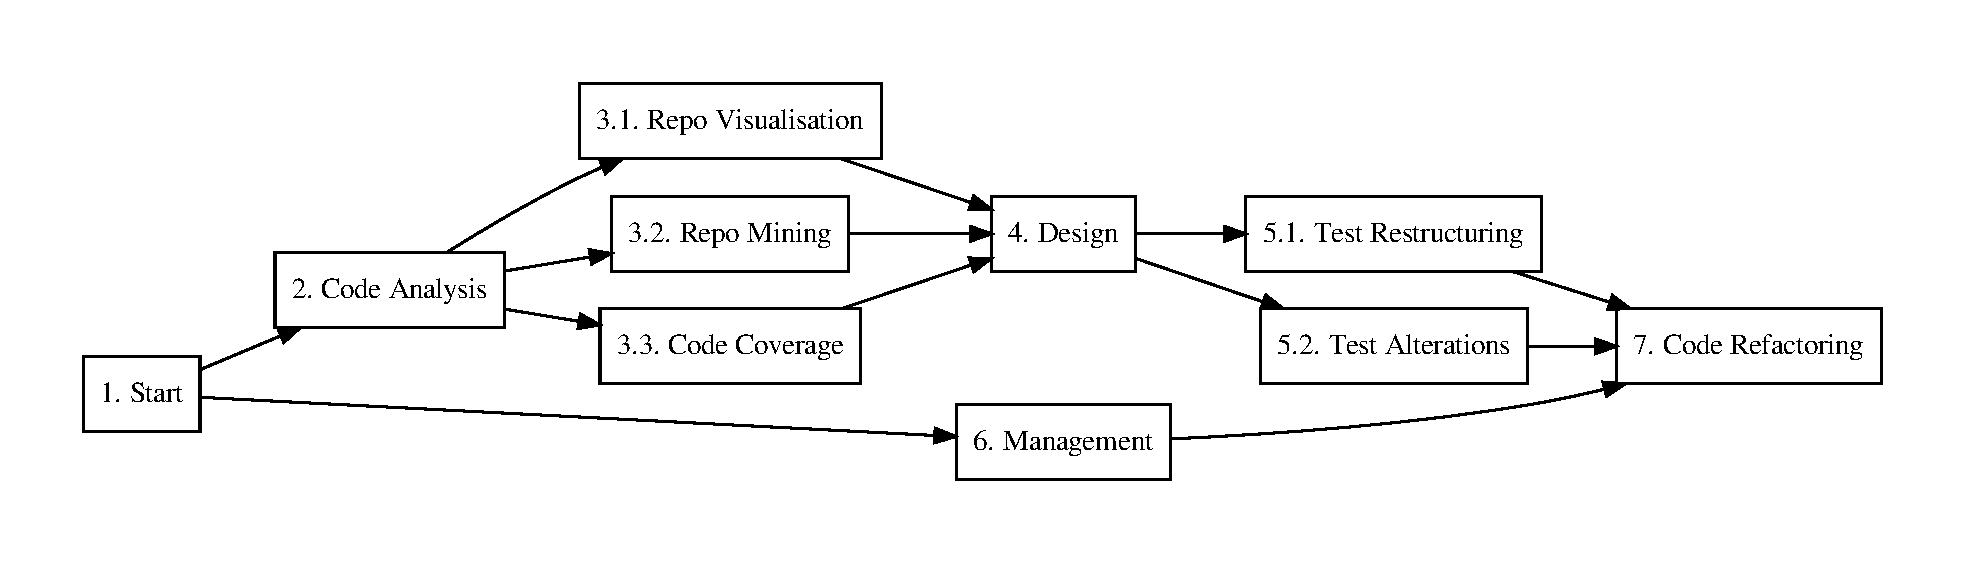
\includegraphics[width=\textwidth]{pert.pdf}
		\caption{Simplified PERT-Chart for the Refactoring of \texttt{JFreeChart}} 
		\label{pert} 
	\end{figure} 
   
	In order for us to cleanly work on the reengineering of \texttt{JFreeChart}, we decided to make a \textsf{PERT}-chart \cite{pert}, as you can see in \textsl{Fig.\,\ref{pert}}. This is a simplified model, without annotations of any critical tasks, paths, or the latest end dates for each task. 
   
	As you can see, \textsl{Management} is a task we will do throughout the entire process of refactoring the project. Tasks \textsl{3.1. Repo Visualisation}, \textsl{3.2 Repo Mining} and \textsl{3.3 Code Coverage} can be found later in this document, respectively in \textsl{sections \ref{sec:gource}, \ref{sec:codescene}} and \textsl{\ref{sec:coco}}. 
   
	
	\subsection{First Contact}
	Seeing as we don't have any experience with the project, nor with its uses, we tried to get a good, general overview. When trying to \textsl{Read all the Code in One Hour} (3.2 from \cite{demeyer2009object}) and to \textsl{Skim the Documentation} (3.3 from \cite{demeyer2009object}), we found that is was quite the difficult task and although it certainly helped in getting a good understanding of how the system worked, it was far from ideal.
	
	
	\section{Project Analysis and Tool Usage}
	In order to solidly identify the issues with \texttt{JFreeChart} and find possible refactoring targets, we made use of a few helpful tools that allowed for clear identification of possible problem areas. This way we can clearly \textsl{Study the Exceptional Entities} (4.3 from \cite{demeyer2009object}). Even though we know that what we find may be tedious or ambiguous to interpret, we will still make our conclusions based on what we know and expect.
	
	\subsection{Repository Visualization with Gource}
	\label{sec:gource}
	The first tool we made use of was \textsf{Gource} \cite{gource}. It is a clean and fancy piece of software that can turn the history of a git repository into a visual representation. This is useful for a few reasons. First, it allows us to see clearly who the main contributers are. There was no surprise that this was \textsl{David Gilbert}.
	
	A second thing we could deduce from this simulation is that the code was not made using the \textsf{Test Driven Development} methodology. We can clearly see that there are first adaptations to the codebase, before changing the tests.
	
	Thirdly, we can identify the possible points in time when a refactoring stage happened in this project. These are moments when a lot of files are added, removed, or modified; which is highlighted in \textsf{Gource}. Granted, it is possible that some of these changes are due to merging multiple branches together.
	
	We've identified that possible refactorings happened in November 2008 (increase in functionality), March 2013 (update to almost all files), December 2014 (update to almost all files and removal of a lot of files), July 2017 (file tree restructuring) and July 2018 (general changes).
	
	Finally, we can use the resulting visualization to \textsl{Learn from the Past} (5.5 from \cite{demeyer2009object}). We can see which classes were changed a lot and which ones remained untouched for the main bulk of the development.
	
	Classes that changed a lot most likely indicate that they are coupled to other classes in the system, marking these classes as important in understanding the general feel of the system.
	
	Classes that remained mainly untouched could indicate abandoned code, but let's assume another possibility. Let's say that these classes indicate features or functionality that are complete. Usually these features cannot give a good enough representation of what's important in the system and whatnot. In either case of untouched code, we can remove our focus from these classes.
	
	\subsection{Repository Mining with CodeScene}
	\label{sec:codescene}
	Another tool we made use of was \textsf{CodeScene} \cite{codescene}, the powerful visualization tool using \textit{Predictive Analytics} to find hidden risks and social patterns in your code.
	
	\textsf{CodeScene} allowed us to get a general feel of the current state of \texttt{JFreeChart}. It gave us a clear representation of possible refactoring targets (see \textsl{attachment \pageref{refactoring-overview}}) and hotspots (see \textsl{attachment \pageref{hotspots-overview}}) within the code\footnote{Please refer to the attachments at the end of this document.}.
	
	When we take a deeper look into the code (or at least the graphical representation thereof), we can identify that we most probably will need to take a look at the \texttt{org.jfree.chart.renderer} package (see \textsl{attachment \pageref{hotspots-package-renderer}}) and the \texttt{org.jfree.chart.plot} package (see \textsl{attachment \pageref{hotspots-package-plot}}), as far as the hotspots are concerned.
	
	On the topic of refactoring targets, it is clear that the \texttt{org.jfree.chart.plot} package (see \textsl{attachment \pageref{refactoring-package-plot}}) really inquires our attention. More specifically the \texttt{XYPlot} (\textsl{attachment \pageref{refactoring-XYPlot}}), \texttt{CategoryPlot} (\textsl{attachment \pageref{refactoring-CategoryPlot}}), \texttt{PiePlot} (\textsl{attachment \pageref{refactoring-PiePlot}}), \texttt{AbstractXYItemRenderer} (\textsl{attachment \pageref{refactoring-AbstractXYItemRenderer}}) and\\ \texttt{AbstractCategoryItemRenderer} (\textsl{attachment \pageref{refactoring-AbstractCategoryItemRenderer}}) classes. In the attachments, the most complex functions are listed (sorted from high to low complexity). These top functions\footnote{The ones with a red cyclomatic complexity.} are most likely to be refactoring targets.
	
	\subsection{Code Coverage with Cobertura}
	\label{sec:coco}
	Chapter 6.3 of \cite{demeyer2009object} tells us to \textsl{Use a Testing Framework}. Not only is this a good idea in refactoring, but in all software projects in general. JUnit was already available in \texttt{JFreeChart}, so there is no need to change of alter this part of the project. Linked with JUnit was \textsf{Cobertura} \cite{cobertura}, a maven plugin that allows us to check how much code was covered with the available tests.
	
	The overview that is generated from this plugin gives us enough information in order to determine which classes and functions were not covered in the project, also yielding possible missing tests. These missing tests can be seen as a symptom for code requiring refactoring (1.1 from \cite{demeyer2009object}). But as discussed above, we will \textsl{Fix Problems, Not Symptoms} (2.5 from \cite{demeyer2009object}) and more specifically, we will mainly focus on the tests that concern our main refactoring targets.
	
	In general, we can deduce that the code coverage of \texttt{JFreeChart} at this point in time is way below comfortable for us.
	
	We also noticed that there is currently no mutation testing being done on this project. Even though we do realize this would give way too much situations and possibilities to cover, we currently have no idea of how good the tests currently are.
	
	\subsection{IntelliJ/Eclipse}
	Because of the jumbled mess \texttt{JFreeChart} is, we decided to look into some tools that might help with the refactoring process itself. The first one that came to mind (and the one that we used to the biggest extend) were the \textsf{IntelliJ} refactoring functionalities (extracting methods/classes, pulling functions up/down...).
	
	Due to our usage with \textsf{IntelliJ}, we also installed the \textsf{Code Smells Detector} plugin \cite{jetbrains-csd}. Unfortunately, this tool appears to be sort of buggy when actually trying to perform some refactoring from the builtin functionality. This is why we combined this plugin with the \textsf{CodeMetrics} plugin \cite{jetbrains-cm}, so we could obtain a valid annotation on the complexity of some functions that were highlighted by the \textsf{Code Smells Detector}. The functions we found here (mostly) lined up with the one we obtained from \textsf{CodeScene}, giving us additional confirmation.
	
	The \textsf{Eclipse} counterpart of this plugin would be \textsf{JDeodorant} \cite{jdeodorant}, but sadly it was quite confusing to use and the results it produced (extracting a few methods to a superclass, moving a method to the class that is used the most in that method...) were, in our opinion, not helpful whatsoever. This is why we decided to identify most of the methods that needed extracting ourselves first and checking the result again afterwards, to see if we have made a difference.
	
	\subsection{Code Clones with iClones}
	While on the topic of code smells, we also used \textsf{iClones} so we could detect duplicate code and other aspects outside of the IDEs we're using. Seeing \textsf{iClones} has builtin functionality to compare different versions of a project, it allows us to easily compare the code at the start of our refactoring process and at the end\footnote{Although we could easily apply this somewhere in the middle of our refactoring process, we've decided that this information is not entirely useful within the context of what we're trying to obtain.}.
	
	Since the results we obtain from using this software are most useful in comparison over time, we will defer our conclusions to \textsl{section \ref{sec:pb}}.
	
	
	\section{Refactoring}
	\subsection{Design Recovery}
	Trying to identify the problem domain, or more specifically, the functionality that required refactoring was quite tricky. This is mainly due to the high rate of exceptional entities and anomalies we've found while applying the \textsl{Study the Exceptional Entities} pattern (4.3 from \cite{demeyer2009object}). Some of these anomalies\footnote{As we would describe them. In \cite{demeyer2009object} they are not mentioned}, we've listed below.
	\begin{itemize}
		\item Renderers that do not render;
		%\item Inconsistent usage of drawing shapes between classes that inherit from the same base. (e.g. \texttt{drawRect} and \texttt{draw(Rectange)});
		\item Implicit implementation of interfaces due to extension of a class that does not implement the interface;
		\item A mixture of a multitude of design patterns that are not all fully implemented (Abstract Factory, Adapters, Bridges, Model View Controller, Chain of Responsibility, Observers...)
		\item ...
	\end{itemize}

	Now, in order for us to describe our proposed new design of \texttt{JFreeChart}, we must first tell you a little bit more about the current design.

	\subsection{Design}
	\subsection{Management}
	\subsection{Refactoring}
	
	\section{Preserved Behaviour}
	\label{sec:pb}
	Of course, in order to be able to say that our refactoring process was effective, we must compare our results to the original source code. While tools like \textsf{iClones} \cite{iclones} automatically come bundled with a version comparison, others, unfortunately, do not. This is why, for this phase of the project, we decided to jump back and forth to the original version of our project and bundle all of our findings below.
	
	As we described in \textsl{section \ref{sec:coco}}, we've been using the tests from \texttt{JFreeChart}. As you can see, our project still passes on all of them, meaning that we (at least) provide the same functionality as when we started (6.1 and 7.6 from \cite{demeyer2009object}).
	
%	In fact, taking a look at our testing coverage, it's clear to see that the overall coverage went up, which is a good thing. This generally implies that our refactoring caused the tests to cover more code, giving us the information that there is more code that has passed the tests. We know now that the system after refactoring is a little bit more robust than before.
	Taking a look at the code coverage reports from \textsf{Cobertura}, we can clearly see that we have some subtle differences. These changes can be either positive (the percentages went up) or negative (they went down).
	
	For the positive changes in these reports, we know they are a good thing. Generally, this implies the refactoring we've done caused the tests to cover more code, giving us the information that there is more code that has passed the tests.
	
	The negative changes on the other hand can also be seen as favorable. The main reason for this is because we removed some lines of code from these files and placed them elsewhere, while the existing covered functionality remained.

	\clearpage
	\bibliographystyle{plain}
	\bibliography{references}
	
	\section*{Attachments}
	On the following pages, we've included a set of screenshots from \textsf{CodeScene} that are referred to in the previous sections. The attachment number is overlayed over the image.
	
	\clearpage
	\setcounter{page}{1}
	\attachment{hotspots-overview}
	\attachment{hotspots-package-renderer}
	\attachment{hotspots-package-plot}
	\attachment{refactoring-overview}
	\attachment{refactoring-package-plot}
	\attachment{refactoring-list}
	\attachment{refactoring-XYPlot}
	\attachment{refactoring-CategoryPlot}
	\attachment{refactoring-PiePlot}
	\attachment{refactoring-AbstractXYItemRenderer}
	\attachment{refactoring-AbstractCategoryItemRenderer}
	
\end{document}